\documentclass[onecolumn, 10pt, letterpaper, twoside]{article}
\usepackage{hyperref}
\usepackage{graphicx}   % need for figures
\usepackage{geometry}
\geometry{letterpaper, portrait, margin=1in}

\newcommand{\nuc}[2] {$^{#1}$#2}

\begin{document}
\title{The ORCHID and DANG User Guide}
\author{James T. Matta - ORNL}
\date{18 Apr 2017}

\maketitle
\begin{abstract}
DANG, The Detector Array for measuring Neutrons and Gammas, is a heterogeneous array of liquid scintillator detectors, large volume NaI(Tl) detectors, and \nuc{3}{He} detectors. ORCHID, the Oak Ridge Conditions at HFIR DAQ, is a data acquisition system written to take data from DANG and was designed to leverage the concurrency provided by modern multi-core processors. DANG and ORCHID are significant component of the ORNL efforts to characterize the backgrounds present in the area that the PROSPECT antineutrino detector (AD) will sit. This document aims to provide a guide to the usage of DANG and ORCHID.
\end{abstract}
\tableofcontents
\clearpage{}
\section{Prerequisites}
\subsection{Access}
One of the first requirements to usage of DANG and/or ORCHID is physical access to the array. This has several requirements for everyone, plus a few extra hoops for foreign nationals.
\begin{itemize}
\item General Requirements
\begin{itemize}
\item General Employee Access Training for HFIR access
\item Basic Rad Training
\end{itemize}
\item Additional requirements for foreign nationals
\begin{itemize}
\item Addition of buildings 7900, 7970, 7970A, and 7972 to your PAS request. (The administrative assistant who initially set up your PAS request can help you here.)
\end{itemize}
\end{itemize}
Another requirement for usage of DANG and/or ORCHID is computer access. For in person or ORNL internal network access the computer controlling the array, the username is \emph{prospect}. The password for that account can be obtained by speaking with James Matta, \href{mailto:mattajt@ornl.gov}{mattajt@ornl.gov}. To access the the system remotely but from within the ornl internal network issue the following command into a linux terminal \emph{ssh -X prospect@prospect1.phy.ornl.gov} then enter your password. At this point you will be remotely logged in to prospect1.

For remote access from outside the lab or the lab visitor network, because prospect1 is on the internal network as opposed to the open research network, the following requirements need to be met:
\begin{itemize}
\item Obtain a UCAMS three character ID
\begin{itemize}
\item Apply for a UCAMS three character ID. This is a somewhat arcane process. If you are a UTK student your best bet is contacting Anne Gladman and asking how to get the process started. Otherwise, contact James Matta, \href{mailto:mattajt@ornl.gov}{mattajt@ornl.gov}, and he will make inquiries.
\end{itemize}
\item Get login1 added to the list of permissions for your UCAMS three character id. For employees, this can be done by contacting the ORNL Solutions Center, this may be the case for non-employees with a UCAMS password, but if they rebuff you, contact James Matta, \href{mailto:mattajt@ornl.gov}{mattajt@ornl.gov}
\item Contact the ORNL Solutions Center and get an RSA token so that you can login to login1.ornl.gov, there will be a small cost associated with this so make certain Alfredo Galindo-Uribarri, \href{mailto:uribarri@ornl.gov}{uribarri@ornl.gov}, is aware of your doing this.
\end{itemize}

Once you have completed these requirements you can access the acquisition machine remotely by issuing the command \emph{ssh -X 3-char-id@login1.ornl.gov} and then proceeding as if you are on the internal network as shown above.

\subsection{GNU Screen}
\subsubsection{Basic Usage}
ORCHID is typically run within a session of GNU screen. This makes is possible to start ORCHID from nothing without being physically at the terminal and not having ORCHID quit when you log out. However, GNU screen takes some getting used to. This is a very basic introduction to screen, more can be found in any of the numerous online tutorials about screen. I particularly recommend the tutorial at \href{https://www.linode.com/docs/networking/ssh/using-gnu-screen-to-manage-persistent-terminal-sessions}{this site} for further learning.

GNU screen is a terminal multiplexer that allows sessions to persist through logoffs. Commands are issued to screen (instead of the terminal within it) by typing \emph{Ctrl+a} and then typing the letter for the command. Some commands are multi-letter or phrases these are used by typing \emph{Ctrl+a}, then typing \emph{:}, and then typing the multi-letter or phrase command.

To start a fresh screen session simply type \emph{screen} in the terminal, to connect to an already existing screen session type \emph{screen -x} instead. Below is the list of useful screen commands that may encountered in the use of ORCHID and DANG
\begin{itemize}
\item \emph{Ctrl+a} + \emph{:multiuser on}  --  Activate multiuser mode to prevent problems if two people log in to the same screen session. This should be used at screen startup.
\item \emph{Ctrl+a} + \emph{c}  --  Create a new terminal window / 'tab' in the multiplexer.
\item \emph{Ctrl+a} + \emph{\#}  --  Jump to window / 'tab' number \emph{\#}. Screen starts on window / 'tab' \emph{0}. Creating additional windows / 'tabs' gives them increasing numbers from \emph{1} to \emph{9}.
\item \emph{Ctrl+a} + \emph{d}  --  Disconnect from the screen session without closing it.
\item \emph{Ctrl+a} + \emph{k}  --  Kill the current screen window / 'tab'.
\end{itemize}

\subsubsection{Setting Up A Screen Session For ORCHID} 
To set up a screen session to run orchid and the associated monitoring in the following steps need to be followed.
\begin{itemize}
\item[1.] Open a terminal.
\item[2.] Start screen (\emph{screen}).
\item[3.] Turn on multi user mode (\emph{Ctrl+a} + \emph{:multiuser on})
\item[4.] Create five additional screen terminals (\emph{Ctrl+a} + \emph{c} used five times)
\item[5.] Switch to window 0 (\emph{Ctrl+a} + \emph{0})
\item[6.] Navigate to the ORCHID directory (\emph{cd /home/prospect/ORCHID})
\item[7.] Start ORCHID (\emph{./orchid orchid\_cfg}) (more on this later)
\item[8.] Switch to window 1 (\emph{Ctrl+a} + \emph{1})
\item[9.] Navigate to the ORCHID directory (\emph{cd /home/prospect/ORCHID})
\item[10.] Start display of the ORCHID log file (\emph{watch -n 5 "tail -n 30 orchid\_*.log"})
\item[11.] Switch to window 2 (\emph{Ctrl+a} + \emph{2})
\item[12.] Navigate to the ORCHID *data* directory (\emph{cd /media/ORNLData/ORCHID\_Data})
\item[13.] Start display of the ORCHID data directory (\emph{watch -n 5 "ls -lh RUN\_NAME | tail -n 30"})
\item[14.] Switch to window 3 (\emph{Ctrl+a} + \emph{3})
\item[15.] Navigate to the ORCHID *data* directory (\emph{cd /media/ORNLData/ORCHID\_Data})
\item[16.] Switch to window 4 (\emph{Ctrl+a} + \emph{4})
\item[17.] Navigate to the ORCHID directory (\emph{cd /home/prospect/ORCHID})
\item[18.] Switch to window 5 (\emph{Ctrl+a} + \emph{5})
\item[19.] Navigate to the DigitizerTester directory (\emph{cd /home/prospect/DigitizerTester})
\end{itemize}
With these steps done, window 0 is used for running ORCHID, window 1 is used for a continuous display of the ORCHID log file, window 2 is used for the continuous display of the ORCHID Data files, window 3 is used for running commands in the data directory (like transfers to the ORNL cluster), window 4 is used for running commands in the ORCHID directory (like the HV scripts mentioned below), and finally, window 5 can be used to run a program that reads all the settings registers of the digitizer and outputs them (\emph{./digitizerReader}) or a program that clears the settings of the digitizer, which is useful if the program crashed or something (\emph{./digitizerClearer}).

\section{DANG Guide}
\subsection{Introduction}
DANG, pictured on the left of Fig. \ref{fig:DANG-Pic-Layout} is a heterogeneous array consisting of eight large volume NaI(Tl) detectors, eight liquid scintillator detectors (containing NE213 liquid scintillator), and two \nuc{3}{He} neutron detectors, one moderated, and one unmoderated. The bottom two liquid scintillator detectors are normally not connected (NNC). The right of Fig. \ref{fig:DANG-Pic-Layout} shows a clearer layout for DANG, including the NNC liquid scintillator detectors. DANG is mobile and can be moved by unlocking the wheels under the platform and pushing. This will be discussed in somewhat greater detail later.

\begin{figure}[h!]
\begin{center}
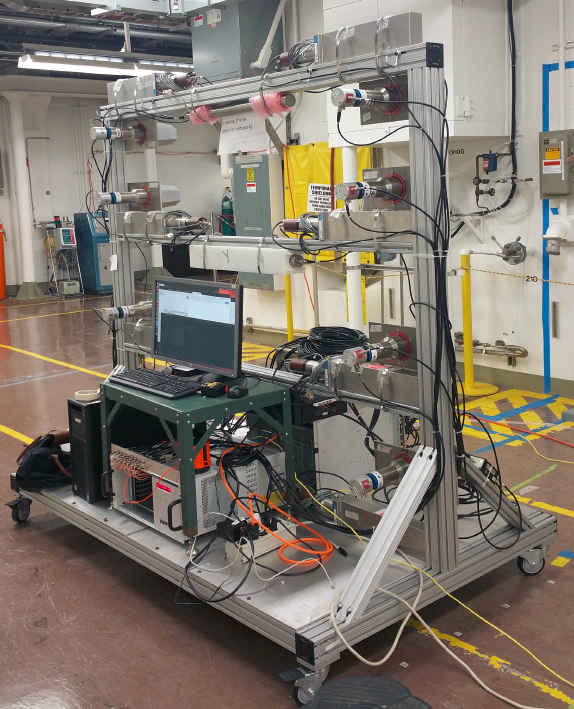
\includegraphics[width=0.35\textwidth]{./DANG_Picture.png}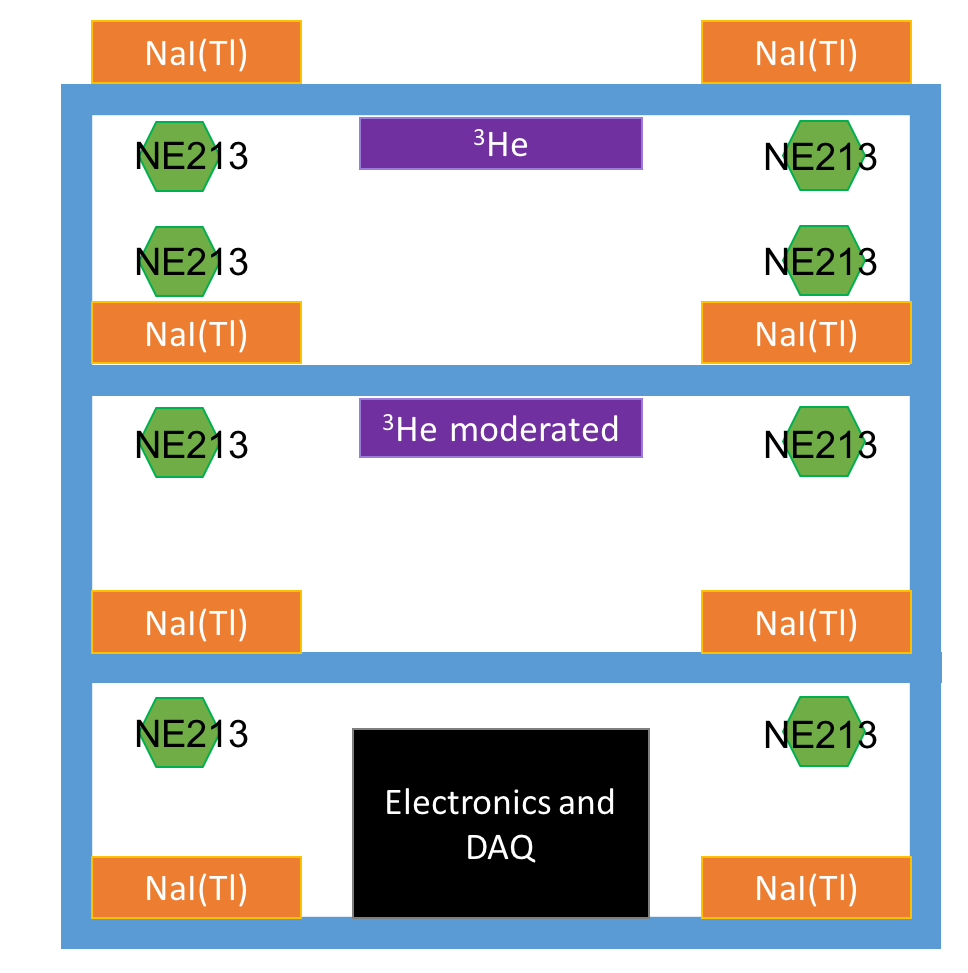
\includegraphics[width=0.4\textwidth]{./DANG_Layout.png}
\caption{Left: Picture of DANG. Right: Diagram of DANG layout}
\label{fig:DANG-Pic-Layout}
\end{center}
\end{figure}

\subsection{Wiring}
Fig. \ref{fig:DANG-Wiring} shows the digitizer and high voltage connections for the DANG detectors. On the left of Fig. \ref{fig:DANG-Wiring} the channel numbers for the VX1730 digitizer are superimposed on the detectors. On the right of Fig. \ref{fig:DANG-Wiring}, the HV channels are superimposed on the detectors shown in the layout. The format for the HV labels is $uXYY$ where $X$ is the module number and $YY$ is the channel number for that module. Module $0$ is the positive voltage module, capable of providing up to $3mA$ at up to $3kV$ on each of its output channels. Module $1$ is the negative voltage model, capable of providing up to $3mA$ at up to $-3kV$ on each of its output channels.

\begin{figure}[h!]
\begin{center}
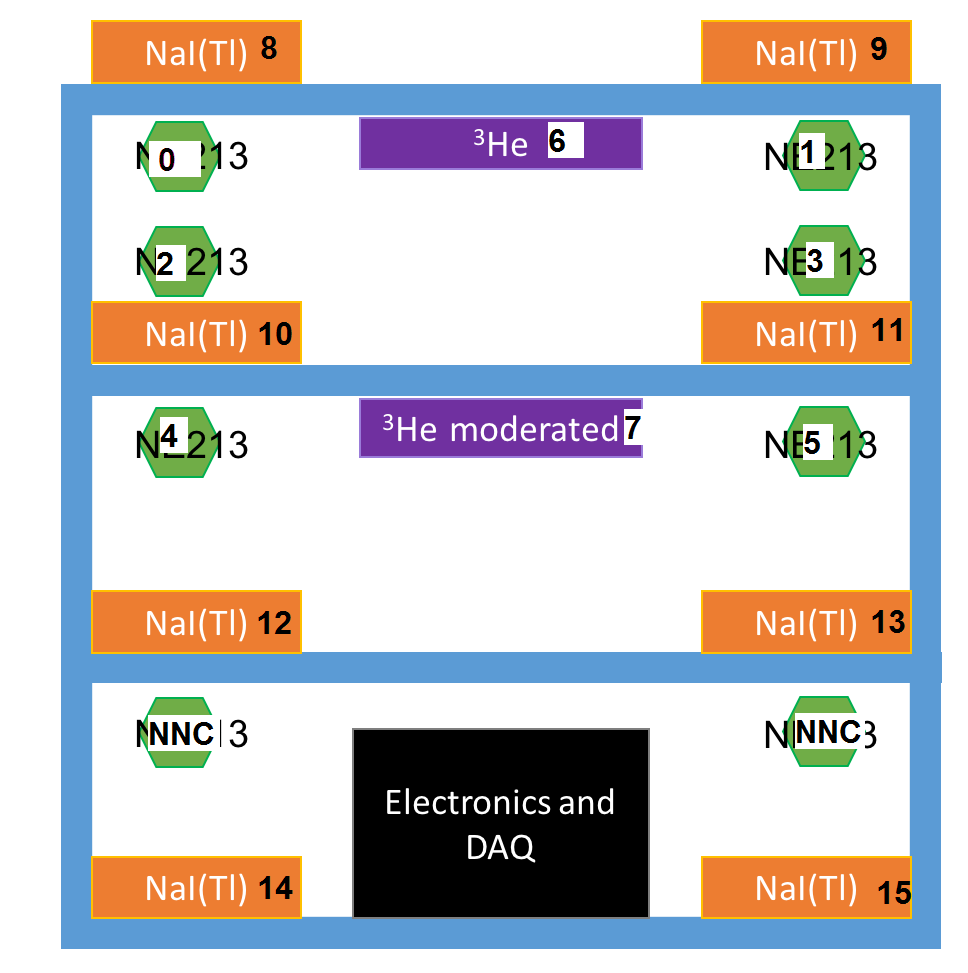
\includegraphics[width=0.4\textwidth]{./DANG_Layout_Digi_Chans.png}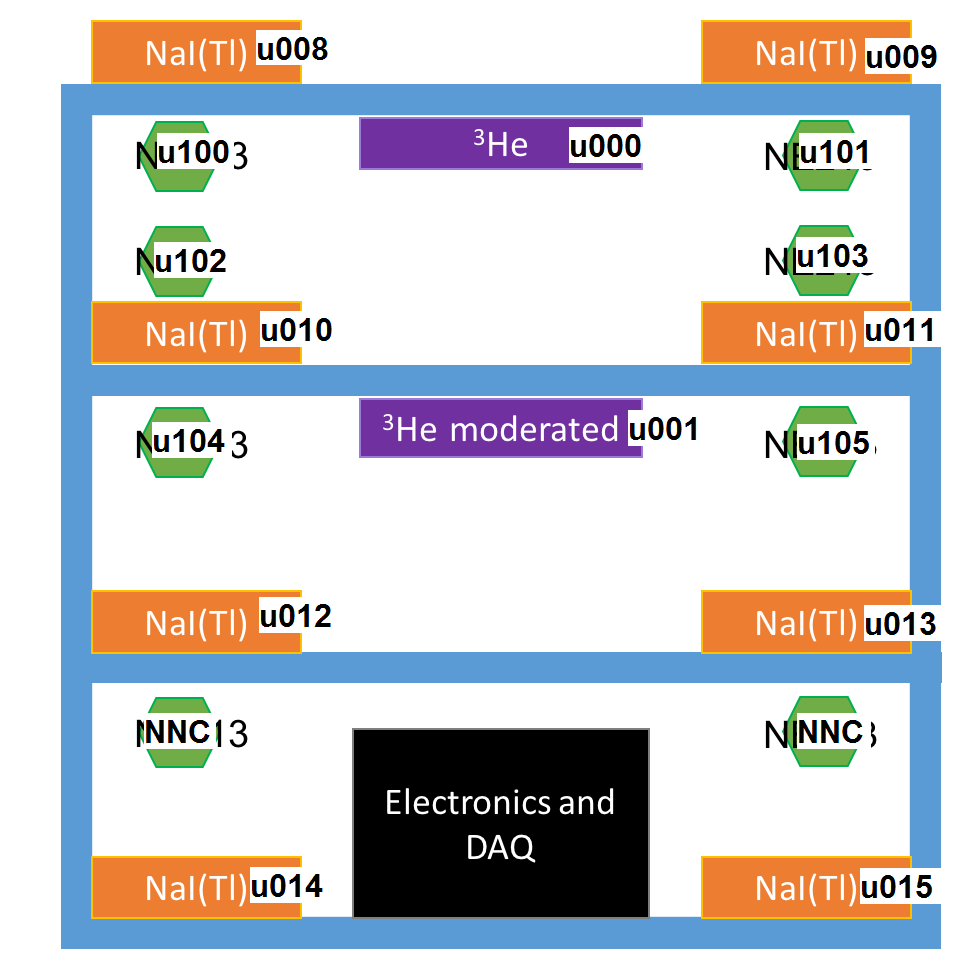
\includegraphics[width=0.4\textwidth]{./DANG_Layout_HV_chans.png}
\caption{Left: Picture of DANG. Right: Diagram of DANG layout}
\label{fig:DANG-Wiring}
\end{center}
\end{figure}

The liquid scintillator and NaI(Tl) detectors all have the anode output of their photo-multiplier tubes directly connected to the input of the VX1730 digitizer. However, the two \nuc{3}{He} detectors must follow a somewhat more complicated signal path. The output from their preamplifiers is connected to a NIM spectroscopic amplifier whose output is them connected to the digitizer. The spectroscopic amplifier shortens the signals from 100 microseconds to about twelve microseconds and converts a positive tail pulse into a negative gaussian pulse.

\subsection{Mobility}
A key feature of DANG is the ability to move the array into a variety of positions, this allows measurements of the background field to be made in a variety of locations to map the spatial background variations.

\subsubsection{Instructions}

To move DANG within a room:
\begin{itemize}
\item Stop data acquisition
\item Unlock the wheels of DANG
\item Move DANG to the desired location, making sure you do not run over trailing power and network cables
\item Lock the wheels
\item Change the data acquisition run-name and run-number
\item Start data acquisition
\end{itemize}

To move DANG to another room (for instance from the ``experiment room'' which will host the PROSPECT AD ``near position'' to the ``MIF room'' which will host the AD ``far position''):
\begin{itemize}
\item Stop data acquisition
\item Shutdown ORCHID
\item Shutdown the HV output
\item Shutdown the computer
\item Turn the VME Crate, NIM Crate, and MPOD Crate off
\item Unplug the network and power connections
\item Unlock the wheels of DANG
\item Move DANG to the desired location, making sure you do not run over trailing power and network cables
\item Lock the wheels
\item Plug in the power connection (and the network connection if there is an available port, there isn't in the MIF room)
\item Start the VME, NIM, and MPOD Crates
\item Start the computer
\item Reset the HV output
\item Start the HV output
\item Start ORCHID
\item Set the data acquisition run-name and run-number
\item Start data acquisition
\end{itemize}

\subsubsection{Positioning}
Positioning of the DANG array is relatively simple. The coordinate system is show in Fig. \ref{fig:Coord-System}. In this coordinate system, the hinge of the back door of the MIF room is the origin. Moving from the origin towards the reactor wall, perpendicular to the wall that the MIF back door is part of, is moving in the positive X direction. Moving from the origin towards the roll-up door, parallel to the wall the MIF back door is part of, constitutes moving in the positive Y direction. With the positive Z direction pointing up a right-handed coordinate system is formed.

\begin{figure}[h!]
\begin{center}
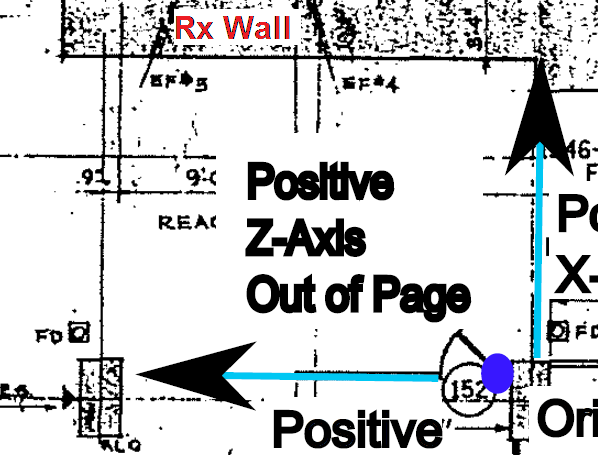
\includegraphics[width=0.5\textwidth]{./Coord_System.png}
\caption{Coordinate system for DANG positioning. The purple dot shows the origin at the hinge of the back door to the MIF room.}
\label{fig:Coord-System}
\end{center}
\end{figure}

Coordinate relative to the origin are measured in inches (because units pain is good for character!). To position DANG at a particular set of coordinates align the center of the outer edge of the right vertical pillar with the location of the coordinate on the floor (as shown in Fig \ref{fig:Positioning-alignment}). While maintaining that alignment, ensure that the long edges of DANG are parallel to the wall with the back door to the MIF room.

\begin{figure}[h!]
\begin{center}
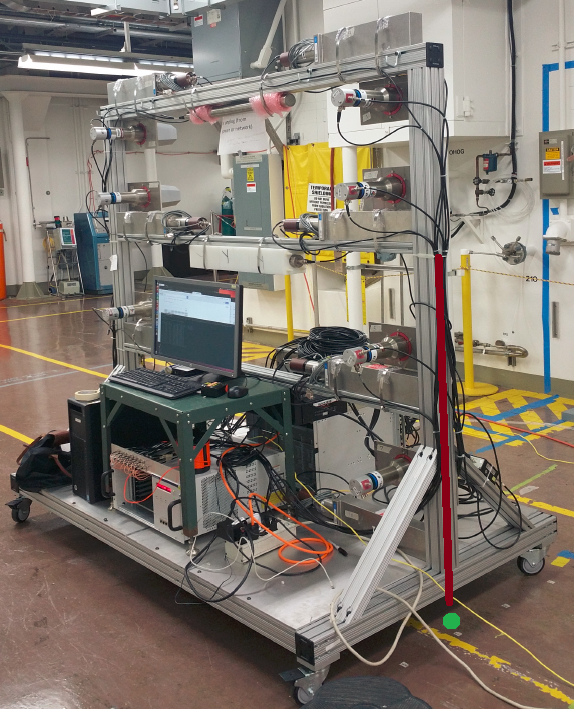
\includegraphics[width=0.375\textwidth]{./Positioning.png}
\caption{Diagram for aligning DANG with a particular set of coordinates.}
\label{fig:Positioning-alignment}
\end{center}
\end{figure}

If the array is aligned in this fashion, with the right side facing the negative Y direction, then the detector center positions relative to the floor coordinates are given in Table \ref{tab:Det-Offsets}.

\begin{table}[h!]
\caption{Detector position offsets, relative to the floor coordinate (X, Y, Z=0) when the coordinate is aligned under the outer edge of the right vertical pillar and the long edges are parallel to the MIF room back wall.\label{tab:Det-Offsets}}
\begin{center}
\begin{tabular}{|l|l|c|c|c|}
\hline
Det. Type & Det. Num. & X Offset & Y Offset & Z Offset \\
\hline
\hline
Liquid Scintillator & 0 & 3.5 & 70.0 & 73.0 \\
Liquid Scintillator & 1 & 3.5 & 9.0 & 73.0 \\
Liquid Scintillator & 2 & 3.5 & 70.0 & 60.0 \\
Liquid Scintillator & 3 & 3.5 & 9.0 & 60.0 \\
Liquid Scintillator & 4 & 3.5 & 70.0 & 38.0 \\
Liquid Scintillator & 5 & 3.5 & 9.0 & 38.0 \\
Unmoderated \nuc{3}{He} & 6 & 0.0 & 39.0 & 75.0 \\
Moderated \nuc{3}{He}& 7 & 0.0 & 39.0 & 50.0 \\
NaI(Tl) & 8 & 0.0 & 68.0 & 81.0 \\
NaI(Tl) (Alt. Base) & 9 & 0.0 & 11.0 & 81.0 \\
NaI(Tl) (Alt. Base) & 10 & 0.0 & 68.0 & 55.0 \\
NaI(Tl) & 11 & 0.0 & 11.0 & 55.0 \\
NaI(Tl) & 12 & 0.0 & 68.0 & 33.0 \\
NaI(Tl) & 13 & 0.0 & 11.0 & 33.0 \\
NaI(Tl) & 14 & 0.0 & 68.0 & 11.0 \\
NaI(Tl) & 15 & 0.0 & 11.0 & 11.0 \\
\hline
\end{tabular}
\end{center}
\end{table}

\clearpage

\subsection{MPOD Usage}
Using the MPOD is most conveniently achieved through a set of scripts in the ORCHID sub-directory of the prospect user's home directory (``/home/prospect/ORCHID'', frequently referred to as ``~/ORCHID''). Running the script \emph{resetHV.sh} will set the maximum currents and voltages  to sane values for all the channels, send reset error condition signals to all the channels, and ensure that all the channels outputs are turned off.
Running the script \emph{startHV.sh} will set the output voltages to the values selected for all the detectors in the array (assuming the detectors are wired as shown in the right of Fig \ref{fig:DANG-Wiring}) and turn the outputs on. Running the script \emph{stopHV.sh} will set all the detector voltages to 0 volts and deactivate all outputs. Finally \emph{statHV.sh} will print out the current measurement of Terminal Voltages, Sense Voltages and Output Currents for all the channels. Below is a quick summary of these commands.

\begin{itemize}
\item \emph{startHV.sh} -- Turn on all used voltage channels and set their values as appropriate for the attached detectors.
\item \emph{stopHV.sh} -- Turn off all used voltage channels and set their values to zero.
\item \emph{statHV.sh} -- Print voltages and currents for all channels.
\item \emph{resetHV.sh} -- Reset current and voltage limits, reset error conditions, ensure that all channels are off.
\end{itemize}

Table \ref{tab:DANG-Power-Information} contains the set voltages and expected currents for each detector that is currently in DANG.

\begin{table}[hb!]
\caption{Detector position offsets, relative to the floor coordinate (X, Y, Z=0) when the coordinate is aligned under the outer edge of the right vertical pillar and the long edges are parallel to the MIF room back wall.\label{tab:DANG-Power-Information}}
\begin{center}
\begin{tabular}{|l|c|c|c|}
\hline
Det. Type & Det. Num. & Set Voltage & Typical Current \\
\hline
\hline
Liquid Scintillator & 0 & $1240V$ & $405.0\mu{}$ \\
Liquid Scintillator & 1 & $1240V$ & $404.0\mu{}$ \\
Liquid Scintillator & 2 & $1240V$ & $404.0\mu{}$ \\
Liquid Scintillator & 3 & $1240V$ & $405.0\mu{}$ \\
Liquid Scintillator & 4 & $1240V$ & $405.0\mu{}$ \\
Liquid Scintillator & 5 & $1240V$ & $405.0\mu{}$ \\
Unmoderated \nuc{3}{He} & 6 & $1700V$ & $0.0\mu{}$ \\
Moderated \nuc{3}{He}& 7 & $1700V$ & $0.0\mu{}$ \\
NaI(Tl) & 8 & $1000V$ & $187.0\mu{}$ \\
NaI(Tl) (Alt. Base) & 9 & $1200V$ & $359.0\mu{}$ \\
NaI(Tl) (Alt. Base) & 10 & $1200V$ & $359.0\mu{}$ \\
NaI(Tl) & 11 & $1000V$ & $185.0\mu{}$ \\
NaI(Tl) & 12 & $1000V$ & $185.0\mu{}$ \\
NaI(Tl) & 13 & $1000V$ & $186.0\mu{}$ \\
NaI(Tl) & 14 & $1000V$ & $186.0\mu{}$ \\
NaI(Tl) & 15 & $1000V$ & $187.0\mu{}$ \\
\hline
\end{tabular}
\end{center}
\end{table}

\clearpage
\section{ORCHID Guide}
ORCHID is a multi-threaded data acquisition system built on the boost, ncurses, and CAENComm libraries. It pipelines the acquisition by having a thread which manages pulling data from the digitizer, multiple threads to process the digitizer data blocks into individual events, a thread to query/monitor the MPOD system (and any other slow controls systems that may come later), a thread to manage user display and control, and finally a thread to take events and slow controls data and write it to disk.

\subsection{Configuration Files}
There are five configuration files for ORCHID. These configuration files contain a good deal of comments (lines starting with a \#) explaining the input information within them. A brief explanation of each file follows.

The primary configuration file (usually called ``orchid\_cfg'') stores a few basic settings. The path to the output directory for the data written. The number of processing threads to create, the number of times per second that the UI thread should update, the paths to the two digitizer configuration files, the paths to the two MPOD configuration files, the MPOD IP address, the slow controls polling rate, the MPOD SNMP support file, and options for if ORCHID should attempt to power on and power off the MPOD HV channels itself.

The MPOD module configuration file (usually called ``orchid\_mpod\_mod\_params.csv'') is a csv that contains a line for every MPOD module that needs to be queried / controlled by ORCHID. The data here is simple, which modules are on and off, maximum voltages and currents, current trip times, what the module number is (set by slot number), etc.

The MPOD channel configuration file (usually called ``orchid\_mpod\_chan\_params.csv'') is a csv that contains a line for every MPOD module channel combination that needs to be queried / controlled by ORCHID. The data here is simple, module number, channel number, ramp rate, voltage set point current set point, and maximum time that current can be exceeded in milliseconds.

The digitizer module configuration file (usually called ``orchid\_digitizer\_mod\_params.csv'') is a csv that contains a line for every VX1730 digitizer module that needs to be queried / controlled by ORCHID. Unlike the HV configuration, you cannot break any equipment with this file, but you might ``break'' the data that we extract from DANG. There are a *lot* of entries in this file. I do my best in the comments of the file to explain what these options are, if you are in doubt contact James Matta, \href{mailto:mattajt@ornl.gov}{mattajt@ornl.gov}.

The digitizer channel configuration file (usually called ``orchid\_digitizer\_chan\_params.csv'') is a csv that contains a line for every VX1730 digitizer channel that needs to be queried / controlled by ORCHID. Unlike the HV configuration, you cannot break any equipment with this file, but you might ``break'' the data that we extract from DANG. There are a *lot* of entries in this file. I do my best in the comments of the file to explain what these options are, if you are in doubt contact James Matta, \href{mailto:mattajt@ornl.gov}{mattajt@ornl.gov}.

\subsection{Starting ORCHID}
Once everything is connected and the HV is started, starting ORCHID is simple. Simply type \emph{./orchid orchid\_cfg} in the command line of window 0 in the screen session (as stated in the instructions for screen.) As ORCHID starts it will regurgitate the input files it read onto the screen as seen in Figs. \ref{fig:ORCHID_Startup1}, \ref{fig:ORCHID_Startup2}, \ref{fig:ORCHID_Startup3}, \ref{fig:ORCHID_Startup4}, and \ref{fig:ORCHID_Startup5}.
\begin{figure}[h!]
\begin{center}
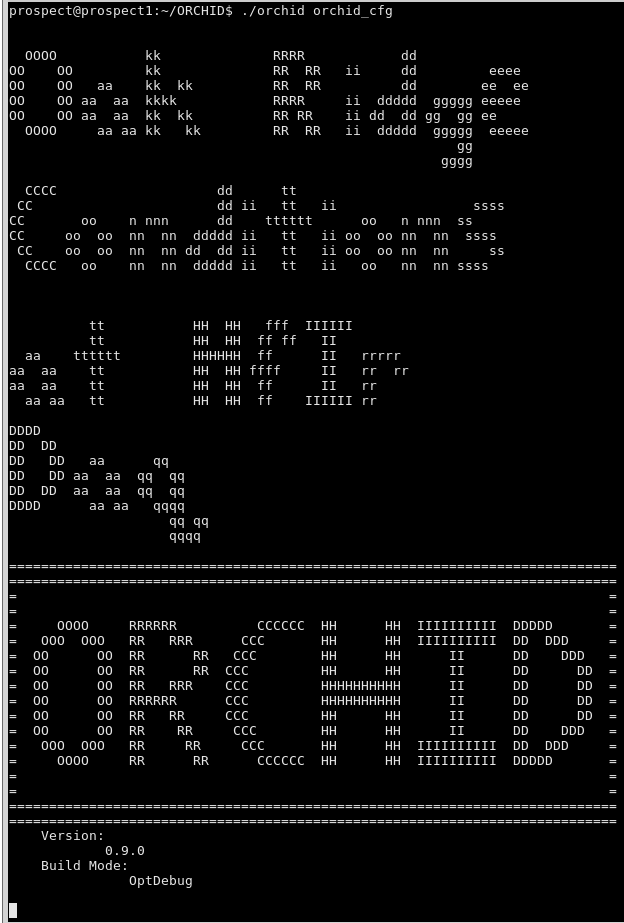
\includegraphics[width=\textwidth]{./Start_Screen_1.png}
\caption{ORCHID output at startup}
\label{fig:ORCHID_Startup1}
\end{center}
\end{figure}
\begin{figure}[h!]
\begin{center}
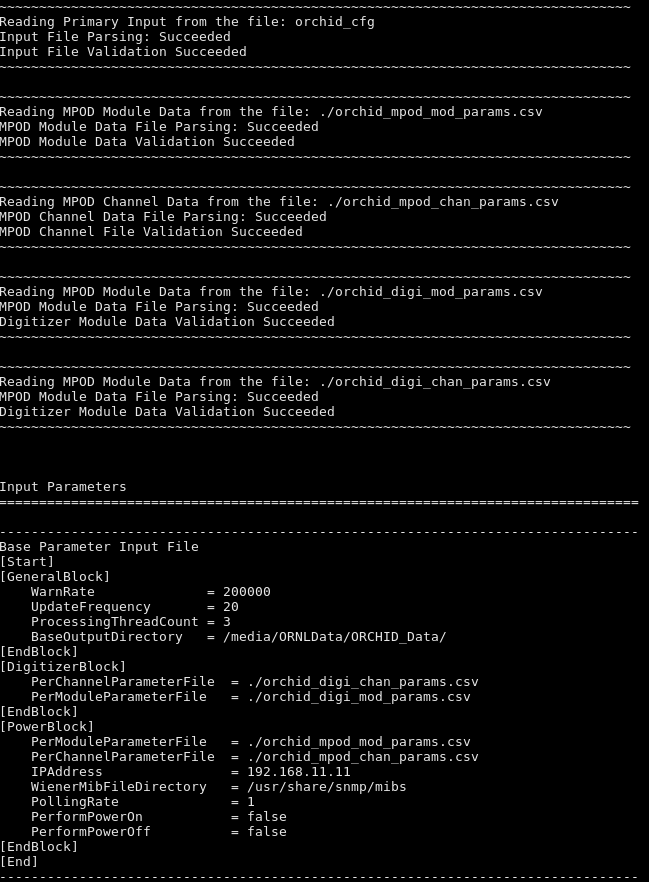
\includegraphics[width=\textwidth]{./Start_Screen_2.png}
\caption{ORCHID output at startup}
\label{fig:ORCHID_Startup2}
\end{center}
\end{figure}
\begin{figure}[h!]
\begin{center}
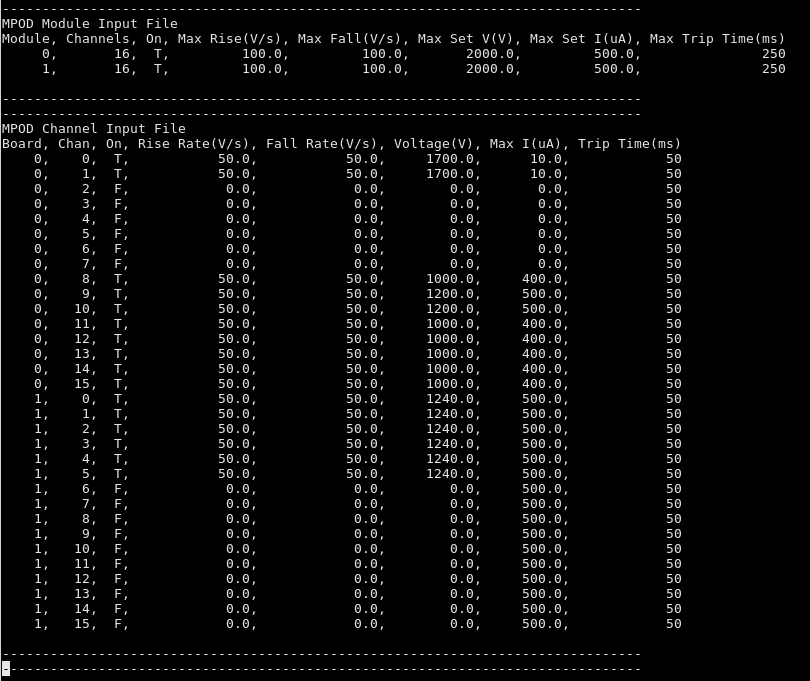
\includegraphics[width=\textwidth]{./Start_Screen_3.png}
\caption{ORCHID output at startup}
\label{fig:ORCHID_Startup3}
\end{center}
\end{figure}
\begin{figure}[h!]
\begin{center}
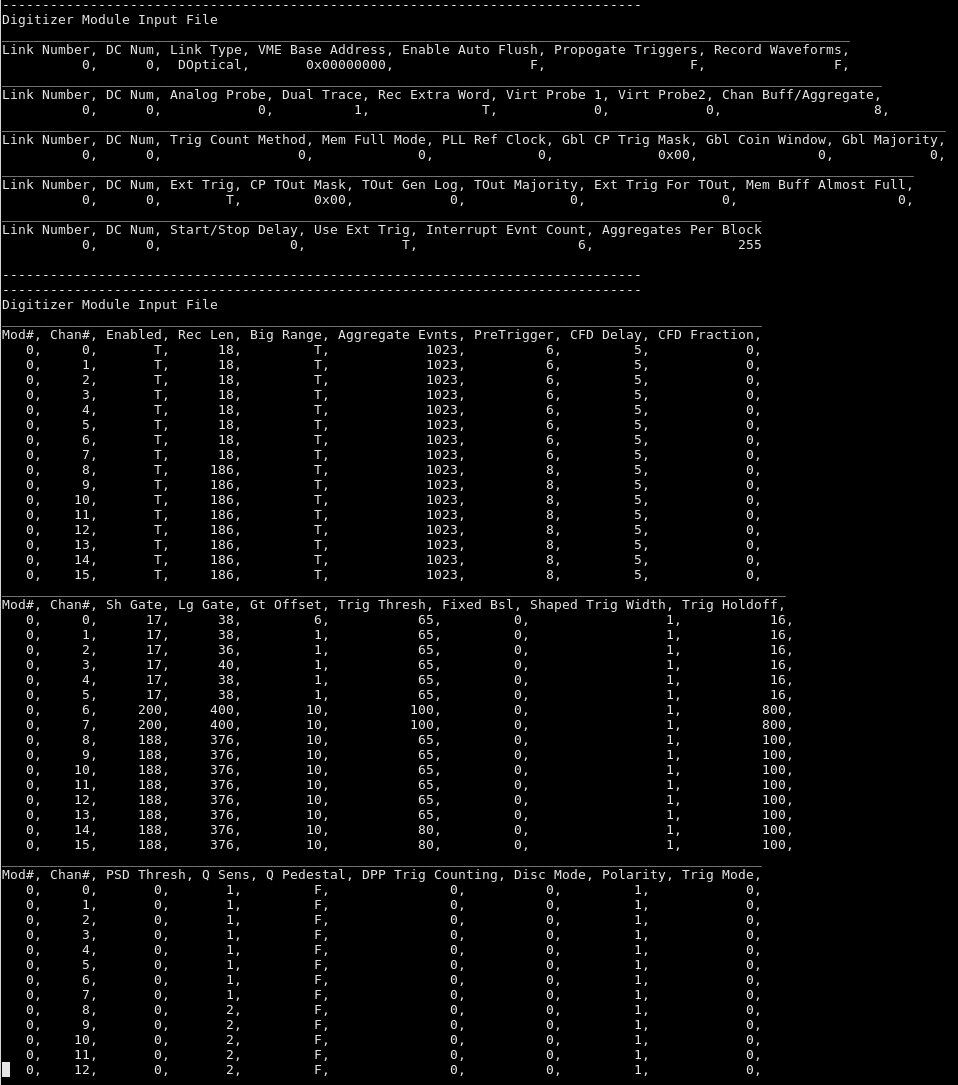
\includegraphics[width=\textwidth]{./Start_Screen_4.png}
\caption{ORCHID output at startup}
\label{fig:ORCHID_Startup4}
\end{center}
\end{figure}
\begin{figure}[h!]
\begin{center}
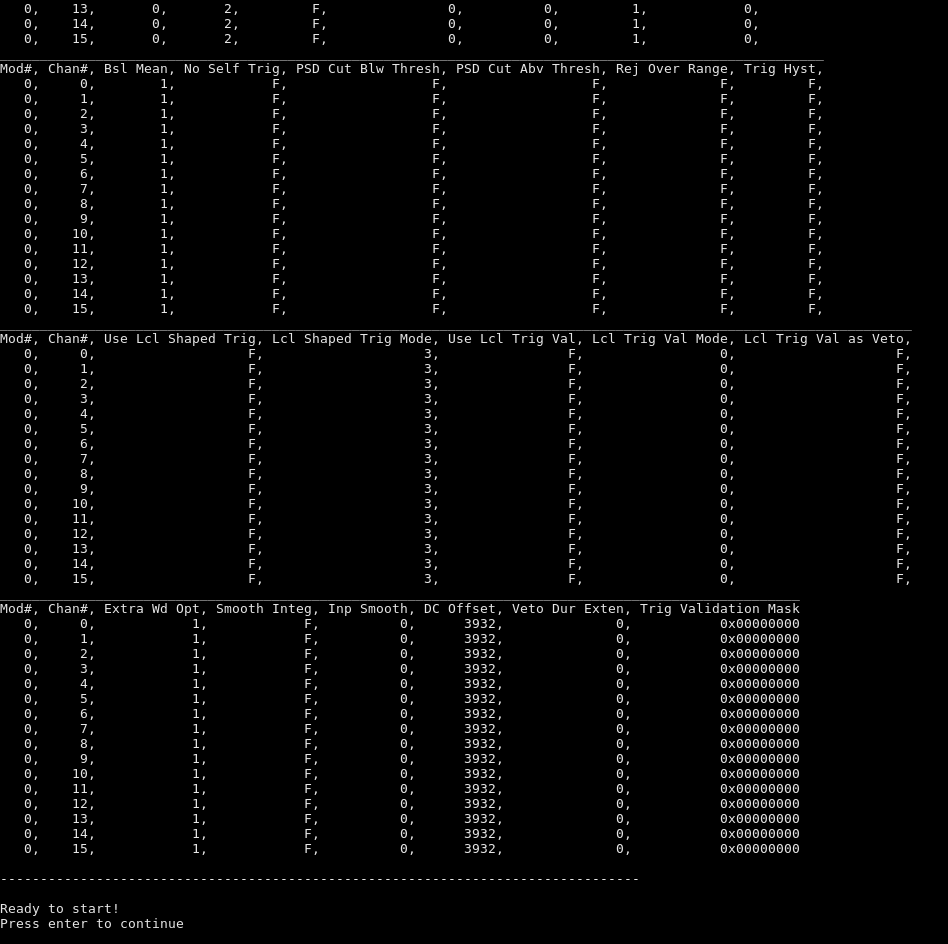
\includegraphics[width=\textwidth]{./Start_Screen_5.png}
\caption{ORCHID output at startup}
\label{fig:ORCHID_Startup5}
\end{center}
\end{figure}

Once it has displayed this you can press \emph{enter} to proceed with starting orchid or \emph{Ctrl+c} to quit if, on review, you find a parameter is incorrect.
\clearpage{}
\subsection{The ORCHID ``Power Up'' Screen}
This screen (seen in Fig. \ref{fig:ORCHID_Powerup}) allows the user to type one of two commands. ``turnon'' will turn the HV system if the general configuration file option "PerformPowerOn" is set to True, otherwise it simply takes you to the ``Main'' menu. ``quit'' and ``exit'' will make ORCHID quit.
\begin{figure}[h!]
\begin{center}
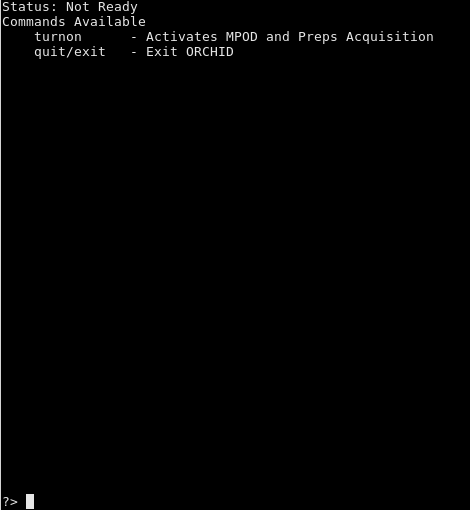
\includegraphics[width=\textwidth]{./Powerup_Menu.png}
\caption{ORCHID power up screen}
\label{fig:ORCHID_Powerup}
\end{center}
\end{figure}

\subsection{The ORCHID ``Main'' Screen}
This screen (seen in Fig. \ref{fig:ORCHID_Main}) allows the user to start acquisition, change run titles, run numbers, turn off HV (returning you to the ``Power Up'' Screen), or quit. Below is a summary of the commands and their actions.

\begin{figure}[h!]
\begin{center}
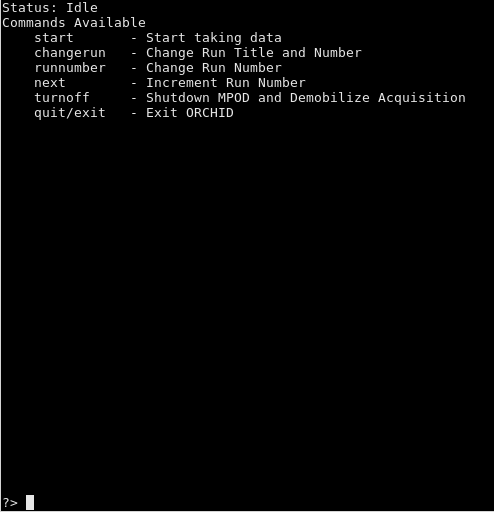
\includegraphics[width=\textwidth]{./Main_Menu.png}
\caption{ORCHID main screen}
\label{fig:ORCHID_Main}
\end{center}
\end{figure}

\begin{itemize}
\item The `start` command starts data acquisition and slow controls event writing. It then transitions to the 'Data Taking Screen.' On program startup the `start` command will not work until the `changerun` command has been used to set both the run title and run number. On subsequent returns to this screen after the first, `start` will not work until *at least* the run number has been changed, using either then `runnumber` or `next` commands.
\item The `changerun` command allows the user to change both the run title and run number.
\item The `runnumber` command allows the user to change the run number to an arbitrary value.
\item The `next` command allows the user to increment the run number from its current value.
\item The `turnoff` command varies with the option "PerformPowerOff" as well. If "PerformPowerOff" is set to "False", it will simply take the user back to the 'Initialize HV Screen'. If it is set to "True" ORCHID will ramp down the MPOD HV and set the MPOD to off, then go to the 'Initialize HV Screen'
\item The `quit` command functions exactly as expected, however its exact behavior will vary somewhat with the "PerformPowerOff" option. If it is set to "False" ORCHID will immediately exit. If "PerformPowerOff" is set to "True" then, before exitting, the quit command will cause ORCHID to ramp the MPOD channels to 0V then sends the "Main power off" signal prior to exitting.
\end{itemize}

\subsection{The ORCHID ``Running'' Screen}
The running screen (seen in Fig. \ref{fig:ORCHID_Running}) is primarily an information display. It shows: trigger rates and counts for each channel on the digitizer, the run title, run number, file name, file path, and MPOD voltage and current readings. It should be noted that the HV readings are not in the same order as the digitizer channels. One needs to keep in mind the mapping between detector number and HV channel show on the right of Fig. \ref{fig:DANG-Wiring}. There are two commands available here though. ``stop'' will cease acquisition and return to the ``Main'' Screen. ``quit'' will stop acquisition, power the MPOD system off (if "PerformPowerOff" is set to true in the configuration file), and exit ORCHID.

\begin{figure}[h!]
\begin{center}
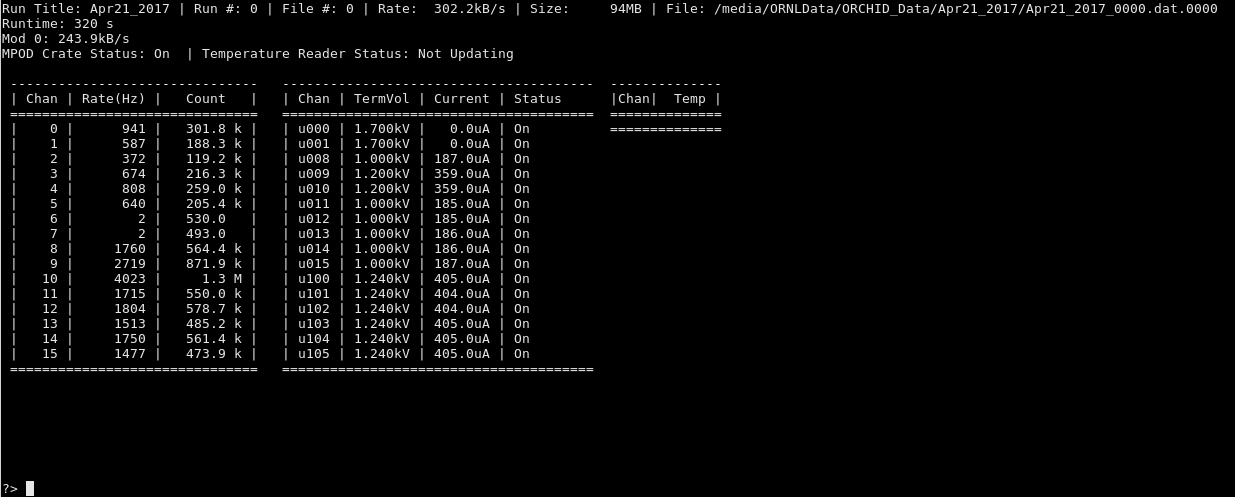
\includegraphics[width=\textwidth]{./Running_Screen.png}
\caption{ORCHID running screen}
\label{fig:ORCHID_Running}
\end{center}
\end{figure}
\end{document}